There are two strategies involving assumptions. One adds assumptions and the other rearranges them. Assumptions represent catalytic variable and are usually used to track number of points in cells. 

Let $\mathcal{T}_1 = ((2,1),\set{12^{(0,0)},1^{(0,0)}23^{(1,0)},123^{(1,0)}},\emptyset)$ and suppose $\mathcal{T}_2$ is $\mathcal{T}_1$ with the assumption that we can count the number of points in $(0,0)$ as shown in \FigureRef{fig:addassumption}. Let $T_1(x)$ and $T_2(x,y)$ be the generating function for $\mathcal{T}_1$ is $\mathcal{T}_2$ respectively, then $T_1(x) = x^0 + 2x^1 + 5x^2 + 14x^3 + 42x^4 + \dotsm$ while $T_2(x,y)$ is
\begin{align*}
    &\ x^0y^0\\
    + &\ x^1y^0 + x^1y^1\\
    + &\ 2x^2y^0 + 2x^2y^1 + x^2y^2\\
    + &\ 5x^3y^0 + 5x^3y^1 + 3x^3y^2 + x^3y^3\\
    + &\ 14x^4y^0 + 14x^4y^1 + 9x^4y^2 + 4x^4y^3 + x^4y^4\\
    + &\ \dotsm  
\end{align*}
and $T_1(x) = T_2(x,1)$.

\begin{figure}[ht!]
    \centering
    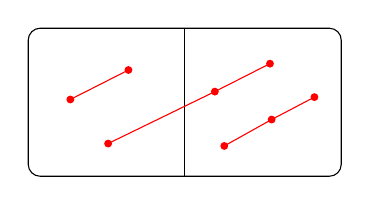
\begin{tikzpicture}[scale=.5, every node/.style={scale=1}]
        \def\xscale{1.0} % Horizontal scale factor
        \def\yscale{1.0} % Vertical scale factor
        \def\spnt{0.1} % Size of smaller points
        \def\lpnt{0.125} % Size of larger points
        \def\roundscale{0.5} % The rounding factor
        \draw[rounded corners=2ex*\roundscale] (0,0) rectangle (7.95*\xscale,3.76*\yscale);
        \draw (3.975*\xscale, 3.76*\yscale) -- (3.975*\xscale, 0);
        \fill[red] (1.07*\xscale, 1.95*\yscale) circle (\spnt);
        \fill[red] (2.54528714910204*\xscale, 2.6989467166405166*\yscale) circle (\spnt);
        \draw[red] (1.07*\xscale, 1.95*\yscale) -- (2.54528714910204*\xscale,2.6989467166405166*\yscale);
        \fill[red] (2.0293687843386805*\xscale, 0.8303608518652064*\yscale) circle (\spnt);
        \fill[red] (4.74*\xscale, 2.15*\yscale) circle (\spnt);
        \fill[red] (6.14*\xscale, 2.86*\yscale) circle (\spnt);
        \draw[red] (2.0293687843386805*\xscale, 0.8303608518652064*\yscale) -- (4.74*\xscale,2.15*\yscale) -- (6.14*\xscale,2.86*\yscale);
        \fill[red] (4.98*\xscale, 0.77*\yscale) circle (\spnt);
        \fill[red] (6.182673140408181*\xscale, 1.4407267632510294*\yscale) circle (\spnt);
        \fill[red] (7.27*\xscale, 2.01*\yscale) circle (\spnt);
        \draw[red] (4.98*\xscale, 0.77*\yscale) -- (6.182673140408181*\xscale,1.4407267632510294*\yscale) -- (7.27*\xscale,2.01*\yscale);
\end{tikzpicture}
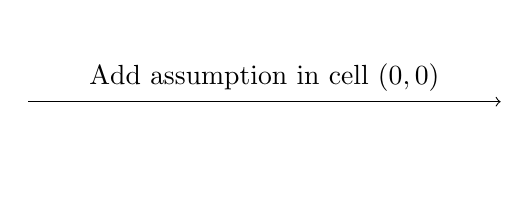
\begin{tikzpicture}[scale=0.5]
    \fill[white] (0,0) rectangle (1,3.76);
    \draw[->] (-5.5,3.76*.5) -- (6.5,3.76*.5) node[above,pos=.5] {Add assumption in cell $(0,0)$};
\end{tikzpicture}
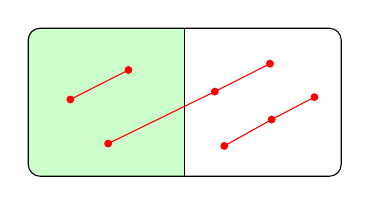
\begin{tikzpicture}[scale=.5, every node/.style={scale=1}]
        \def\xscale{1.0} % Horizontal scale factor
        \def\yscale{1.0} % Vertical scale factor
        \def\spnt{0.1} % Size of smaller points
        \def\lpnt{0.125} % Size of larger points
        \def\roundscale{0.5} % The rounding factor
        \fill[green!20, rounded corners=2ex*\roundscale] (0,0) rectangle (1*\xscale,3.76*\yscale);
        \fill[green!20] (0.5*\xscale,0) rectangle (3.975*\xscale,3.76*\yscale);
        \draw[rounded corners=2ex*\roundscale] (0,0) rectangle (7.95*\xscale,3.76*\yscale);
        \draw (3.975*\xscale, 3.76*\yscale) -- (3.975*\xscale, 0);
        \fill[red] (1.07*\xscale, 1.95*\yscale) circle (\spnt);
        \fill[red] (2.54528714910204*\xscale, 2.6989467166405166*\yscale) circle (\spnt);
        \draw[red] (1.07*\xscale, 1.95*\yscale) -- (2.54528714910204*\xscale,2.6989467166405166*\yscale);
        \fill[red] (2.0293687843386805*\xscale, 0.8303608518652064*\yscale) circle (\spnt);
        \fill[red] (4.74*\xscale, 2.15*\yscale) circle (\spnt);
        \fill[red] (6.14*\xscale, 2.86*\yscale) circle (\spnt);
        \draw[red] (2.0293687843386805*\xscale, 0.8303608518652064*\yscale) -- (4.74*\xscale,2.15*\yscale) -- (6.14*\xscale,2.86*\yscale);
        \fill[red] (4.98*\xscale, 0.77*\yscale) circle (\spnt);
        \fill[red] (6.182673140408181*\xscale, 1.4407267632510294*\yscale) circle (\spnt);
        \fill[red] (7.27*\xscale, 2.01*\yscale) circle (\spnt);
        \draw[red] (4.98*\xscale, 0.77*\yscale) -- (6.182673140408181*\xscale,1.4407267632510294*\yscale) -- (7.27*\xscale,2.01*\yscale);
\end{tikzpicture}
    \caption{The tiling $((2,1),\set{12^{(0,0)},1^{(0,0)}23^{(1,0)},123^{(1,0)}},\emptyset)$ with and without an assumption.}
    \label{fig:addassumption}
\end{figure}

When the cells of one assumption is a subset of the cells of another we can rearrange them. This is demonstrated for tiling $((3,1),\set{12^{(0,0)},1^{(0,0)}23^{(1,0)},12^{(1,0)}3^{(2,0)}},\emptyset)$ in \FigureRef{fig:assrear} where the left one has $y$ as a catalytic variable for points in $(0,0)$ and $z$ for points in either $(0,0)$ or $(1,0)$ while in the right one $z$ only tracks those in $(1,0)$ after the assumptions have been rearranged. If $T_1(x,y,z)$ is the generating function before the arrangement and $T_2(x,y,z)$ after then $T_1(x,y,z) = T_2(x,yz,z)$.

\begin{figure}[ht!]
    \centering
    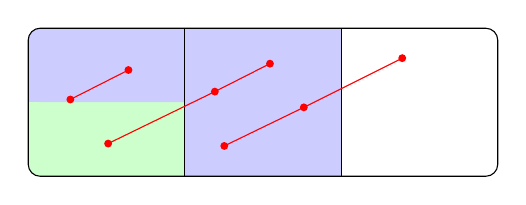
\begin{tikzpicture}[scale=.5, every node/.style={scale=1}]
        \def\xscale{1.0} % Horizontal scale factor
        \def\yscale{1.0} % Vertical scale factor
        \def\spnt{0.1} % Size of smaller points
        \def\lpnt{0.125} % Size of larger points
        \def\roundscale{0.5} % The rounding factor
        
        \fill[green!20, rounded corners=2ex*\roundscale] (0,0) rectangle (1*\xscale,3.76*\yscale*.5);
        \fill[green!20] (0.5*\xscale,0) rectangle (3.975*\xscale,3.76*\yscale*.5);
        \fill[green!20] (0,.5*\yscale) rectangle (3.975*\xscale,3.76*\yscale*.5);
        
        \fill[blue!20, rounded corners=2ex*\roundscale] (0,3.76*\yscale*.5) rectangle (7.95*\xscale,3.76*\yscale);
        \fill[blue!20] (3.97*\xscale,0) rectangle (7.95*\xscale,3.76*\yscale);
        \fill[blue!20] (0,3.76*\yscale*.5) rectangle (3.975*\xscale,3.76*\yscale*0.7);
        \fill[blue!20] (3.975*\xscale,0) rectangle (5*\xscale,3.76*\yscale);
        
        \draw[rounded corners=2ex*\roundscale] (0,0) rectangle (11.925*\xscale,3.76*\yscale);
        \draw (3.975*\xscale, 3.76*\yscale) -- (3.975*\xscale, 0);
        \draw (2*3.975*\xscale, 3.76*\yscale) -- (2*3.975*\xscale, 0);
        \fill[red] (1.07*\xscale, 1.95*\yscale) circle (\spnt);
        \fill[red] (2.54528714910204*\xscale, 2.6989467166405166*\yscale) circle (\spnt);
        \draw[red] (1.07*\xscale, 1.95*\yscale) -- (2.54528714910204*\xscale,2.6989467166405166*\yscale);
        \fill[red] (2.0293687843386805*\xscale, 0.8303608518652064*\yscale) circle (\spnt);
        \fill[red] (4.74*\xscale, 2.15*\yscale) circle (\spnt);
        \fill[red] (6.14*\xscale, 2.86*\yscale) circle (\spnt);
        \draw[red] (2.0293687843386805*\xscale, 0.8303608518652064*\yscale) -- (4.74*\xscale,2.15*\yscale) -- (6.14*\xscale,2.86*\yscale);
        \fill[red] (4.98*\xscale, 0.77*\yscale) circle (\spnt);
        \fill[red] (7*\xscale, 1.75*\yscale) circle (\spnt);
        \fill[red] (9.5*\xscale, 3*\yscale) circle (\spnt);
        \draw[red] (4.98*\xscale, 0.77*\yscale) -- (7*\xscale,1.75*\yscale) -- (9.5*\xscale,3*\yscale);
\end{tikzpicture}
\hspace{0.5cm}
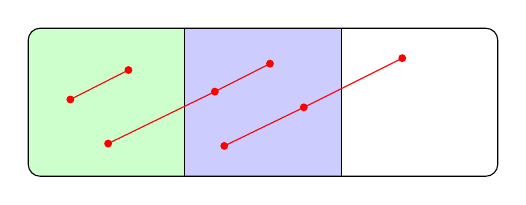
\begin{tikzpicture}[scale=.5, every node/.style={scale=1}]
        \def\xscale{1.0} % Horizontal scale factor
        \def\yscale{1.0} % Vertical scale factor
        \def\spnt{0.1} % Size of smaller points
        \def\lpnt{0.125} % Size of larger points
        \def\roundscale{0.5} % The rounding factor
        \fill[green!20, rounded corners=2ex*\roundscale] (0,0) rectangle (1*\xscale,3.76*\yscale);
        \fill[green!20] (0.5*\xscale,0) rectangle (3.975*\xscale,3.76*\yscale);
        \fill[blue!20] (0+3.975*\xscale,0) rectangle (1*\xscale+3.975*\xscale,3.76*\yscale);
        \fill[blue!20] (0.5*\xscale+3.975*\xscale,0) rectangle (3.975*\xscale+3.975*\xscale,3.76*\yscale);
        \draw[rounded corners=2ex*\roundscale] (0,0) rectangle (11.925*\xscale,3.76*\yscale);
        \draw (3.975*\xscale, 3.76*\yscale) -- (3.975*\xscale, 0);
        \draw (2*3.975*\xscale, 3.76*\yscale) -- (2*3.975*\xscale, 0);
        \fill[red] (1.07*\xscale, 1.95*\yscale) circle (\spnt);
        \fill[red] (2.54528714910204*\xscale, 2.6989467166405166*\yscale) circle (\spnt);
        \draw[red] (1.07*\xscale, 1.95*\yscale) -- (2.54528714910204*\xscale,2.6989467166405166*\yscale);
        \fill[red] (2.0293687843386805*\xscale, 0.8303608518652064*\yscale) circle (\spnt);
        \fill[red] (4.74*\xscale, 2.15*\yscale) circle (\spnt);
        \fill[red] (6.14*\xscale, 2.86*\yscale) circle (\spnt);
        \draw[red] (2.0293687843386805*\xscale, 0.8303608518652064*\yscale) -- (4.74*\xscale,2.15*\yscale) -- (6.14*\xscale,2.86*\yscale);
        \fill[red] (4.98*\xscale, 0.77*\yscale) circle (\spnt);
        \fill[red] (7*\xscale, 1.75*\yscale) circle (\spnt);
        \fill[red] (9.5*\xscale, 3*\yscale) circle (\spnt);
        \draw[red] (4.98*\xscale, 0.77*\yscale) -- (7*\xscale, 1.75*\yscale) -- (9.5*\xscale,3*\yscale);
\end{tikzpicture}
    \caption{By rearranging the assumptions on the left we get the assumptions on the right.}
    \label{fig:assrear}
\end{figure}